\chapter{Выполнение задания}

Далее приведены код алгоритма сортировки подсчетом \cite{sort} и графовые представления для него.

\section{Средства реализации}

Реализация алгоритма сортировки подсчетом выполнялась при помощи языка программирования Python \cite{python}. Выбор ЯП обусловлен простотой синтаксиса.

\section{Программный код}

В листинге \ref{lst:sort} представлен код алгоритма сортировки подсчетом.
\clearpage
\begin{center}
\captionsetup{justification=raggedright,singlelinecheck=off}
\begin{lstlisting}[label=lst:sort,caption=Сортировка подсчетом]
def counting_sort():
    size = int(input("Input size: "))       # 1

    arr = []                                # 2

    for _ in range(size):                   # 3
        arr.append(randint(-10, 10))        # 4

    min_elem = min(arr)                     # 5
    max_elem = max(arr)                     # 6
    
    d = min_elem - 1                        # 7
    add_size = max_elem - min_elem + 1      # 8

    add_arr = [0] * add_size                # 9

    for i in range(size):                   # 10
        j = arr[i] - d - 1                  # 11
        add_arr[j] += 1                     # 12
    
    i = 0                                   # 13

    for j in range(add_size):               # 14
        if add_arr[j] > 0:                  # 15
            for _ in range(add_arr[j]):     # 16
                arr[i] = j + d              # 17
                i += 1                      # 18

    return arr
\end{lstlisting} 
\end{center}

\section{Графовые представления}

На рисунке \ref{img:operational} приведен операционный граф для алгоритма сортировки подсчетом, на рисунке \ref{img:information} - информационый граф, на рисунке \ref{img:operational_history} - граф операционной истории и на рисунке \ref{img:information_history} - граф информационой истории.


\begin{figure}[H]
	\begin{center}
		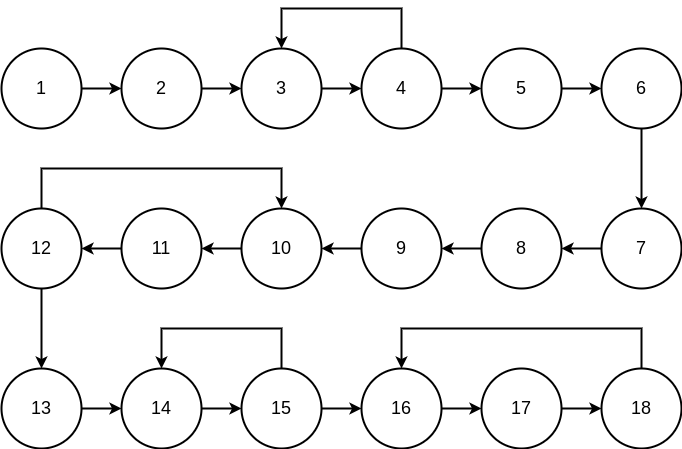
\includegraphics[scale=0.5]{img/operational.png}
	\end{center}
	\captionsetup{justification=centering}
	\caption{Операционный граф}
	\label{img:operational}
\end{figure}

\begin{figure}[H]
	\begin{center}
		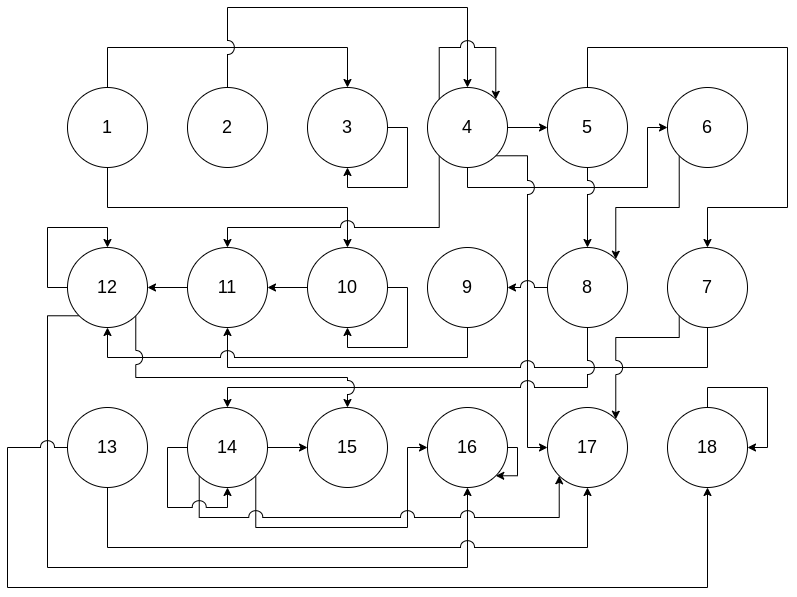
\includegraphics[scale=0.5]{img/information.png}
	\end{center}
	\captionsetup{justification=centering}
	\caption{Информационный граф}
	\label{img:information}
\end{figure}

\begin{figure}[H]
	\begin{center}
		
\includegraphics[scale=0.3]{img/operational_history.png}
	\end{center}
	\captionsetup{justification=centering}
	\caption{Граф операционной истории}
	\label{img:operational_history}
\end{figure}

\begin{figure}[H]
	\begin{center}
		
\includegraphics[scale=0.3]{img/information_history.png}
	\end{center}
	\captionsetup{justification=centering}
	\caption{Граф информационной истории}
	\label{img:information_history}
\end{figure}